\documentclass[conference]{IEEEtran}
\IEEEoverridecommandlockouts
\usepackage{cite}
\usepackage{amsmath,amssymb}
\usepackage{graphicx}
\usepackage{booktabs}
\usepackage{multirow}
\usepackage{xcolor}
\usepackage{url}
\usepackage{tikz}
\usetikzlibrary{arrows.meta,positioning,fit}
\usepackage[hidelinks]{hyperref}
\definecolor{kblue}{HTML}{2A78D6}
\definecolor{kgray}{HTML}{898781}
\newcommand{\ours}{KAN-H}

\begin{document}

\title{Hindsight-Supervised Kolmogorov--Arnold Gates for Interpretable Agentic Control of Training Jobs}

\author{\IEEEauthorblockN{Avanish Kasar, Rupali Biradar, Viverun}
\IEEEauthorblockA{A. P. Shah Institute of Technology (APSIT), Thane, India\\
avanishkasar57@gmail.com}}

\maketitle

\begin{abstract}
Deciding when to stop or re-tune a running training job is usually left to a person watching a loss curve or to a scheduler whose decisions cannot be inspected. We present KAN-KubeAgent, an agentic training controller in which every proposed action must pass through a Kolmogorov--Arnold Network (KAN) gate whose edges are fixed to symbolic functions, so the formula shown to the operator is exactly the function that makes the decision. We identify two problems with training such a gate: imitating a hand-written rule caps it at that rule's quality, and relabelling live runs with the gate's own decisions is circular. We replace both with \emph{hindsight supervision}: each decision point of a completed run is labelled by the validation-loss improvement that actually remained. On 36 real Fashion-MNIST runs spanning six learning rates, two batch sizes and three seeds, evaluated with seed-grouped cross-validation, the hindsight-trained gate saves 31.0\% of the epoch budget at 0.20\% mean regret in best validation loss, against 4.4\% savings for the same gate trained on rule labels and 0.18\% regret for a hindsight oracle. It matches a well-tuned patience rule and linear or MLP gates trained on the same labels, while its decisions are reproducible from a closed-form expression to within $6.5\times10^{-4}$ score points. In closed-loop control of 12 held-out live runs, including real learning-rate changes, the full system saves 37.1\% of epochs with no significant change in best validation loss. We release the system, data and benchmark.
\end{abstract}

\begin{IEEEkeywords}
Kolmogorov--Arnold networks, early stopping, interpretable machine learning, LLM agents, training orchestration
\end{IEEEkeywords}

\section{Introduction}
Fine-tuning and training jobs consume compute long after they stop improving. In practice they are supervised either manually, by an engineer reading loss curves, or automatically, by early-stopping and multi-fidelity schedulers such as Hyperband~\cite{li2018hyperband}, ASHA~\cite{li2020asha} and the median stopping rule~\cite{golovin2017vizier}. Automatic schedulers save compute, but the reason a particular job was stopped is a rank or a bandit statistic rather than an argument a person can check. Large language model (LLM) agents are now being applied to the same space~\cite{zhang2023llmhpo,liu2024agenthpo,huang2024mlagentbench}, which adds natural-language rationales but no guarantee that the rationale is what produced the action.

For high-stakes decisions, Rudin argues for models that are interpretable by construction rather than black boxes explained after the fact~\cite{rudin2019stop}. Kolmogorov--Arnold Networks (KANs)~\cite{liu2025kan} place learnable univariate functions on edges and can be converted to symbolic formulas~\cite{liu2024kan2}, which makes them a natural candidate for an inspectable controller. This paper asks whether a KAN can serve as the binding decision layer of an agentic training controller, and what it should be trained on.

\textbf{Contributions.}
\begin{enumerate}
\item A working system in which LLM-assisted agents observe a real training process and propose actions, and a symbolic KAN gate makes every binding decision (continue, adjust learning rate, early stop). After training, each edge is fixed to a symbolic function, so the displayed formula \emph{is} the decision function; we measure this faithfulness directly.
\item \emph{Hindsight supervision} for the gate: decision points of completed real runs are labelled by the improvement that actually remained, replacing imitation of a hand-written rule and the circular practice of relabelling runs with the gate's own decisions.
\item A benchmark on 36 real learning curves with seed-grouped cross-validation, comparing the gate with patience rules~\cite{prechelt2012early}, the median stopping rule, successive halving, the hand-written rule, and linear, tree and MLP gates trained on the same labels, plus closed-loop runs in which the gate controls live training.
\end{enumerate}
We report where the KAN does not win: in our setting a linear gate trained on the same labels is statistically indistinguishable on regret, which locates the KAN's value in exact, non-linear auditability rather than accuracy.

\section{Related Work}
\textbf{Early stopping and multi-fidelity optimisation.} Patience-based stopping on a validation signal is the classical baseline~\cite{prechelt2012early}. Hyperband~\cite{li2018hyperband} and its asynchronous variant ASHA~\cite{li2020asha} allocate resources across many configurations by successive halving; BOHB adds Bayesian proposals~\cite{falkner2018bohb}; population-based training adapts hyperparameters during training~\cite{jaderberg2017pbt}. Google Vizier's median stopping rule stops a trial whose best objective is worse than the median of other trials' running averages~\cite{golovin2017vizier}. Learning-curve extrapolation predicts final performance from a partial curve, using parametric ensembles~\cite{domhan2015extrapolation}, Bayesian neural networks~\cite{klein2017lcnet} or prior-data fitted networks~\cite{adriaensen2023lcpfn}. These systems are implemented in Optuna~\cite{akiba2019optuna}, Ray Tune~\cite{liaw2018tune} and Kubernetes-native Katib~\cite{george2020katib}. None exposes the decision of a single job as a closed-form expression that executes it.

\textbf{LLM agents for ML engineering.} ReAct-style agents interleave reasoning and tool calls~\cite{yao2023react}. LLMs have been used to propose hyperparameters~\cite{zhang2023llmhpo,liu2024agenthpo}, and benchmarks such as MLAgentBench~\cite{huang2024mlagentbench} and MLE-bench~\cite{chan2025mlebench} measure agents on end-to-end ML tasks. In these systems the agent's output is the action; our design separates proposal from decision.

\textbf{Symbolic and KAN-based interpretability.} Symbolic regression has been used to explain hyperparameter-performance relationships after optimisation~\cite{segel2023symbolic} and to distil learned optimisers~\cite{zheng2022symbolicl2o}. KANs have produced interpretable controllers, e.g.\ an interpretable load-balancing policy in reinforcement learning~\cite{singh2025kanrl}. A controlled comparison finds MLPs generally match or beat KANs except on symbolic-formula tasks~\cite{yu2024kanormlp}, which our results echo. Our gate also resembles a \emph{shield}~\cite{alshiekh2018shielding}: a component that monitors a learner's actions and can override them, here with a learned symbolic rule rather than a temporal-logic specification.

\section{System Design}
\begin{figure}[t]
\centering
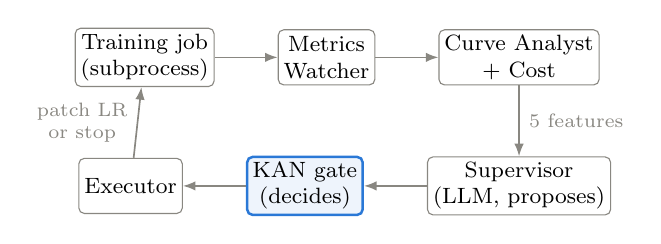
\begin{tikzpicture}[font=\footnotesize, node distance=8mm,
  box/.style={draw=kgray, rounded corners=2pt, minimum height=7mm, align=center, inner sep=2pt},
  key/.style={box, draw=kblue, line width=0.9pt, fill=kblue!8},
  arr/.style={-{Latex[length=1.6mm]}, kgray, line width=0.6pt}]
\node[box] (job) {Training job\\(subprocess)};
\node[box, right=of job] (mw) {Metrics\\Watcher};
\node[box, right=of mw] (an) {Curve Analyst\\+ Cost};
\node[box, below=9mm of an] (sup) {Supervisor\\(LLM, proposes)};
\node[key, left=of sup] (gate) {KAN gate\\(decides)};
\node[box, left=of gate] (ex) {Executor};
\draw[arr] (job) -- (mw);
\draw[arr] (mw) -- (an);
\draw[arr] (an) -- node[right, font=\scriptsize]{5 features} (sup);
\draw[arr] (sup) -- (gate);
\draw[arr] (gate) -- (ex);
\draw[arr] (ex) -- node[left, font=\scriptsize, align=center]{patch LR\\or stop} (job);
\end{tikzpicture}
\caption{Control loop. Agents observe the job and propose an action; the KAN gate's decision is binding, is executed by patching the learning rate or stopping the job, and is logged with the formula that produced it.}
\label{fig:arch}
\end{figure}

\textbf{Control loop.} Fig.~\ref{fig:arch} shows the loop, implemented as a LangGraph state graph. A training job runs as a separate process and reports per-epoch training loss, global gradient norm, learning rate, and validation loss and accuracy. Every $k=2$ epochs from epoch 4, the Metrics Watcher reads the job's state, the Loss-Curve Analyst and Cost Estimator compute five features, and the Supervisor (an LLM) proposes an action with a rationale. The KAN gate scores the same features and its decision is the one executed; agreement or override is logged. The Executor halves the learning rate (or applies the LLM's suggested value) through a file the training process re-reads each epoch, or terminates the process. Control is asynchronous: training continues while agents deliberate, so a decision takes effect at the next epoch boundary the process reaches. The same client interface wraps a Kubeflow TrainJob; in this paper all runs are local processes.

\textbf{Features.} All features lie in $[0,1]$ and are computed only from the past. With monitored (validation) loss $\ell_1,\dots,\ell_t$ and window $w=5$: \emph{loss plateau} $=1-\min(1, 10\,\Delta_w/\ell_{t-w+1})$, where $\Delta_w$ is the non-negative drop over the window; \emph{gradient trend}, the mean gradient norm over the window divided by the run's maximum so far (scale-free across models); \emph{LR-decay benefit}, the fraction of sign changes in successive loss differences over the window (oscillation); \emph{budget remaining}, the unused fraction of the epoch budget; and \emph{epochs since improvement}, divided by 30.

\textbf{Gate.} The gate is a pykan KAN~\cite{liu2025kan,liu2024kan2} of width $[5,3,1]$ with grid 5 and cubic splines, trained with $L_1$ and entropy sparsity regularisation and pruned. It regresses a stop score $s\in[0,100]$, mapped to decisions by fixed bands: continue if $s<40$, adjust learning rate if $40\le s<75$, early stop if $s\ge75$. After training, every active edge is replaced by its best symbolic fit from $\{x, x^2, x^3, \sin\}$ (pykan's \texttt{auto\_symbolic}); the network then evaluates only those symbolic functions, and the formula extracted from it is the exact decision function rather than an approximation of a spline network.

\textbf{Operation.} A dashboard streams the run, each agent step as it completes, hardware telemetry, and each decision traced through the network: every edge's learned function, its value for the current input, and per-feature contributions. Contributions are computed by occlusion against a zero baseline; they are exact when all layers after the first are linear, and the interface reports whether this holds for the deployed gate.

\section{Hindsight Supervision}
\label{sec:hindsight}
The gate was first trained, as in our initial design, on synthetic curves labelled by a three-rule reference policy. A student trained this way can at best reproduce its teacher. A natural fix, harvesting live runs and retraining on them, is circular when the labels are the gate's own decisions: it is self-distillation and adds no information.

We instead label each decision point of a completed run by what actually happened next. Let $b_t=\min_{\tau\le t}\ell_\tau$ be the best monitored loss after $t$ epochs and $b^\ast=\min_{\tau\le T}\ell_\tau$ the best within the full budget $T$. The remaining relative gain and the hindsight stop score are
\begin{equation}
g_t=\frac{b_t-b^\ast}{b_t},\qquad
s^{\mathrm{H}}_t=100\cdot\mathrm{clip}\!\left(1-\frac{g_t}{\tau},\,0,\,1\right),
\end{equation}
where the tolerance $\tau$ (5\% by default) is the relative improvement still worth paying for. With the gate's bands, $s^{\mathrm{H}}_t\ge75$ means less than $\tau/4=1.25\%$ improvement remains. Future information is used only to build labels; at decision time the gate sees only causal features. Runs that the gate itself stopped are right-censored and are excluded from retraining, so harvested live runs contribute labels only when they completed.

\section{Experimental Setup}
\textbf{Workload.} A small CNN (two convolutional and two fully connected layers, 105,866 parameters) is trained with Adam on the first 4,000 Fashion-MNIST~\cite{xiao2017fashion} training images for a budget of $T=40$ epochs, with validation loss and accuracy computed every epoch on 2,000 images of the official test split. We train every combination of learning rate $\{10^{-4},3\cdot10^{-4},10^{-3},3\cdot10^{-3},10^{-2},3\cdot10^{-2}\}$, batch size $\{64,256\}$ and seed $\{0,1,2\}$, without intervention, giving 36 complete curves (1,440 epochs, mean 2.35\,s per epoch on a 4-core CPU without GPU). The grid yields slowly converging, overfitting and unstable runs; the best validation epoch has median 19 and is reached before epoch 20 in 18 of 36 runs. Best validation accuracy ranges up to 88.7\%.

\textbf{Protocol.} Stopping policies are evaluated by counterfactual replay: a policy stopping after epoch $t$ is credited with the best validation loss among the first $t$ epochs (best-checkpoint retention). Learned gates use 3-fold cross-validation grouped by seed, so no test run and no run sharing its initialisation is seen in training; each fold has 432 training decision points. Each learned gate is trained with three seeds and we report mean $\pm$ standard deviation. Offline replay cannot evaluate \emph{adjust LR}, which changes the future curve, so it is treated as \emph{continue} here and measured in closed loop (Section~\ref{sec:closed}).

\textbf{Policies.} No stopping; patience $p\in\{3,5,8\}$ on validation loss; the median stopping rule with training-fold runs as the completed-trial population; synchronous successive halving ($\eta=3$, rungs at 4, 12, 36 epochs), the core of Hyperband and ASHA; the hand-written reference rule; the KAN trained on that rule's labels (``KAN-T'', the original design); and, on hindsight labels, a ridge-regression gate, a depth-3 regression tree, a $32{\times}32$ MLP and our KAN (``\ours''). The hindsight oracle stops at the first decision point where $g_t\le1.25\%$.

\textbf{Metrics.} \emph{Compute saved}: unused share of the epoch budget. \emph{Regret}: $(b_{\text{stop}}-b^\ast)/b^\ast$, the relative loss of best validation loss; we report mean and 90th percentile, the drop in validation accuracy at the best checkpoint, and the \emph{premature} rate, the share of runs with regret above 2\%. Paired differences over the 36 runs use the Wilcoxon signed-rank test.

\section{Results}
\subsection{Per-run efficiency}
\begin{table}[t]
\centering
\caption{Per-run results on 36 held-out real runs (mean $\pm$ std over three gate seeds; deterministic policies have no spread). Regret is the relative increase in best validation loss.}
\label{tab:main}
\setlength{\tabcolsep}{3pt}
\begin{tabular}{lrrrr}
\toprule
Policy & Saved \% & Regret \% & P90 \% & Prem. \% \\
\midrule
No early stopping & 0.0 & 0.00 & 0.00 & 0.0 \\
Patience-3 & 45.1 & 2.38 & 9.21 & 30.6 \\
Patience-5 & 36.3 & 0.62 & 2.97 & 13.9 \\
Patience-8 & 30.6 & 0.24 & 0.00 & 5.6 \\
Median stopping rule & 22.5 & 40.19 & 149.49 & 25.0 \\
Reference rule (teacher) & 33.9 & 2.12 & 9.55 & 25.0 \\
KAN-T (rule labels) & 4.4$\pm$5.5 & 0.36$\pm$0.51 & 1.22 & 7.4 \\
\midrule
Tree, depth 3 & 40.6 & 0.74 & 2.50 & 13.9 \\
Linear & 35.8 & 0.30 & 0.00 & 5.6 \\
MLP $32{\times}32$ & 34.1$\pm$5.8 & 0.34$\pm$0.12 & 0.55 & 7.4 \\
\textbf{\ours\ (ours)} & \textbf{31.0$\pm$1.0} & \textbf{0.20$\pm$0.13} & \textbf{0.00} & \textbf{5.6} \\
\midrule
Hindsight oracle & 43.1 & 0.18 & 0.79 & 0.0 \\
\bottomrule
\end{tabular}
\end{table}

\begin{figure}[t]
\centering
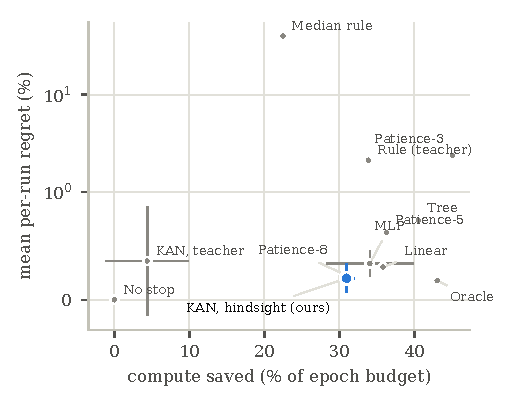
\includegraphics[width=\columnwidth]{figures/pareto.pdf}
\caption{Compute saved against mean regret (symmetric log scale; bars show std over gate seeds). Lower right is better.}
\label{fig:pareto}
\end{figure}

Table~\ref{tab:main} and Fig.~\ref{fig:pareto} summarise per-run results. Hindsight supervision is the decisive change: the same KAN architecture saves 4.4\% of compute when trained on rule labels and 31.0\% when trained on hindsight labels, stopping a median 16 epochs earlier ($p=1.5\times10^{-5}$) with no significant change in regret ($p=0.53$). Its mean regret of 0.20\% is close to the oracle's 0.18\%, its 90th-percentile regret is zero, and the mean accuracy cost at the retained checkpoint is 0.03 percentage points.

\ours\ has significantly lower regret than patience-3 ($p=0.003$) and the reference rule ($p=0.03$). Against patience-5 its regret is not significantly different ($p=0.37$) but it stops later ($p=0.04$), saving less; patience-8 lands at almost the same point (30.6\%, 0.24\%). Linear and MLP gates trained on the same hindsight labels are statistically indistinguishable from \ours\ in regret ($p=0.76$ and $0.75$); the linear gate saves somewhat more compute. The tree saves more but stops prematurely in 13.9\% of runs. The median stopping rule shows why per-run and population objectives differ: it kills configurations that are worse than their peers, so its per-run regret is large by design.

Fig.~\ref{fig:curves} shows three held-out runs. On a slowly converging run all per-run policies train to the budget while the median rule stops it at epoch 4; on an overfitting run \ours\ stops after the minimum has passed but late; on an unstable high-learning-rate run, the case where patience is fastest, \ours\ waits longer.

\begin{figure*}[t]
\centering
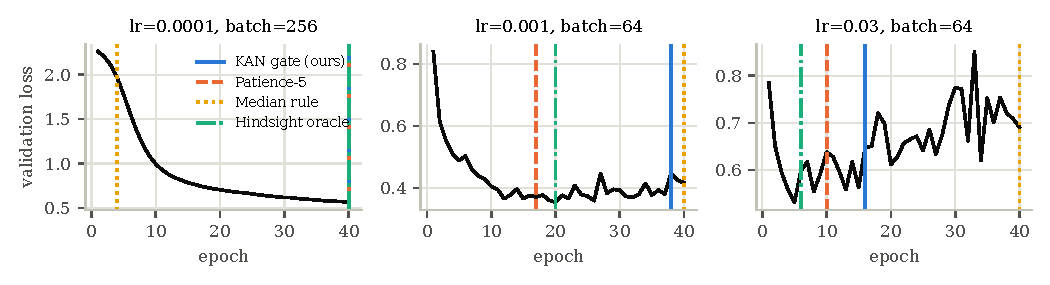
\includegraphics[width=\textwidth]{figures/curves.pdf}
\caption{Validation loss of three held-out runs (seed 2) and where each policy stops.}
\label{fig:curves}
\end{figure*}

\subsection{Population view}
Treating each fold's 12 configurations as one tuning job, successive halving saves 77.5\% of epochs but its best surviving configuration has 3.86\% higher best validation loss than the best available. Per-run policies keep every configuration and therefore find the best one: \ours\ (gate seed 0), linear, patience-5 and patience-8 all reach 0.00--0.01\% best-found regret at 30.6--36.3\% savings. Population schedulers and per-job gates are complementary: halving chooses \emph{which} jobs to continue, the gate decides \emph{when} a job has stopped paying.

\subsection{Decision quality and the cost of symbolic form}
\begin{table}[t]
\centering
\caption{Fit to hindsight targets on held-out decision points (mean over folds and seeds) and interpretability.}
\label{tab:fid}
\setlength{\tabcolsep}{3pt}
\begin{tabular}{lrrrl}
\toprule
Gate & MAE & $R^2$ & Band F1 & Form of decision \\
\midrule
Reference rule & 28.0 & 0.31 & 0.53 & 3 rules \\
KAN-T & 34.5 & 0.21 & 0.29 & formula \\
Tree, depth 3 & 10.6 & 0.79 & 0.71 & 8 leaves \\
Linear & 16.5 & 0.74 & 0.62 & 6 terms \\
MLP & 17.3 & 0.70 & 0.61 & 1,281 weights \\
\ours & 19.0 & 0.71 & 0.60 & $8.4\pm1.2$ terms \\
\bottomrule
\end{tabular}
\end{table}

Table~\ref{tab:fid} reports fit to the hindsight targets. The tree fits best, yet its stepwise output crosses the stop threshold early and costs regret; fit and stopping quality are not the same objective. Converting the KAN to symbolic form has a measurable price: mean validation MAE rises from 12.5 for the spline network to 20.3 after symbolic fixing (nine gates), which is what makes the formula exact. That exactness holds: across the nine \ours\ gates, the largest difference between the extracted formula and the network's output on all test decision points is $6.5\times10^{-4}$ score points on average (the teacher-trained gates: 0.02). Formulas average 24.9 operations over 16.3 active edges. A gate decision takes about 3\,ms, under 0.2\% of an epoch.

The formulas also make the gates auditable as a family. In 8 of the 9 hindsight gates the linear term in gradient trend is negative: a gradient that is still large relative to its peak pushes toward continuing. This kind of cross-seed check is not available from an MLP's weights.

\subsection{The deployed gate}
\begin{figure*}[t]
\centering
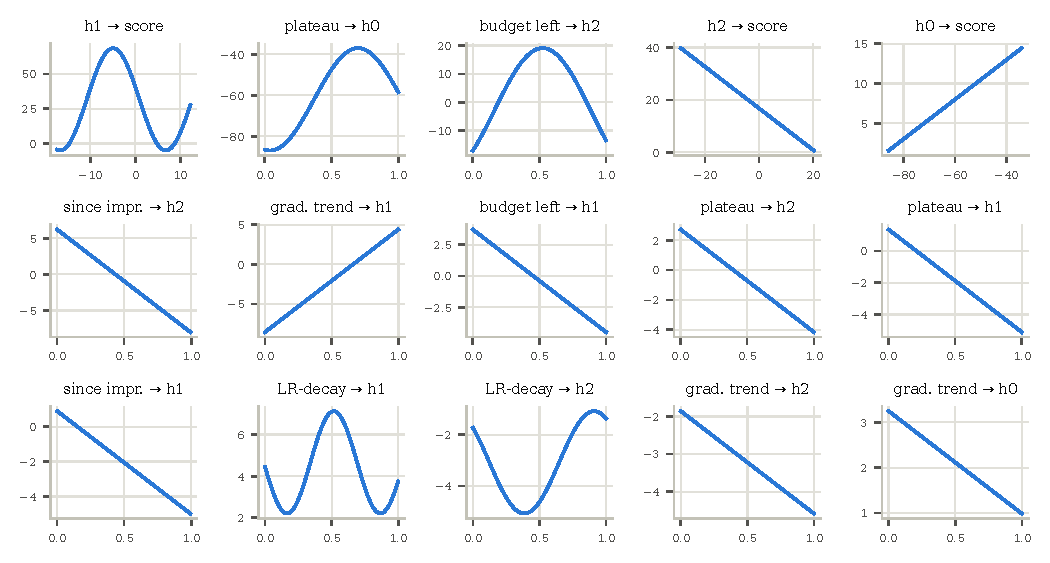
\includegraphics[width=0.9\textwidth]{figures/edges.pdf}
\caption{Every active edge function of the deployed gate (trained on all 36 runs), ordered by learned importance. Each panel is one univariate function; the gate is their composition.}
\label{fig:edges}
\end{figure*}

The deployed gate, trained on all 648 decision points, keeps 15 active edges (Fig.~\ref{fig:edges}). Writing $x_1$ to $x_5$ for plateau, gradient trend, LR-decay benefit, budget remaining and epochs since improvement, its decision function is, with coefficients rounded,
\begin{multline*}
s = 56.0 + 11.3x_5 + 1.6x_2 + 5.5x_1 + 17.4\sin(4.36x_4+8.72)\\
{}+ 6.2\sin(4.76x_1-1.76) - 1.6\sin(5.99x_3+2.40)\\
{}- 36.8\sin(1.59x_5+2.20x_4-3.47x_2+1.73x_1\\
{}+0.66\sin(8.96x_3-6.19)-9.73).
\end{multline*}
The innermost sine comes from a non-linear output-layer edge, so this gate is not additive and its per-feature contributions are occlusion estimates; the formula itself remains exact. For example, after epoch 34 of the learning-rate $10^{-3}$, batch-64 run, the gate scores 100.4 (early stop) from a baseline of 51.1, with the largest occlusion contributions from loss plateau (+68.3) and epochs since improvement (+31.8).

\subsection{Closed-loop control}
\label{sec:closed}
Offline replay cannot show what \emph{adjust LR} does, so we ran the full system, agents and executor included, on the 12 configurations of seed 2 with the gate trained only on seeds 0 and 1, and compared each controlled run with its uncontrolled counterpart (same seed and settings). Fig.~\ref{fig:closed} shows the result.

\begin{figure*}[t]
\centering
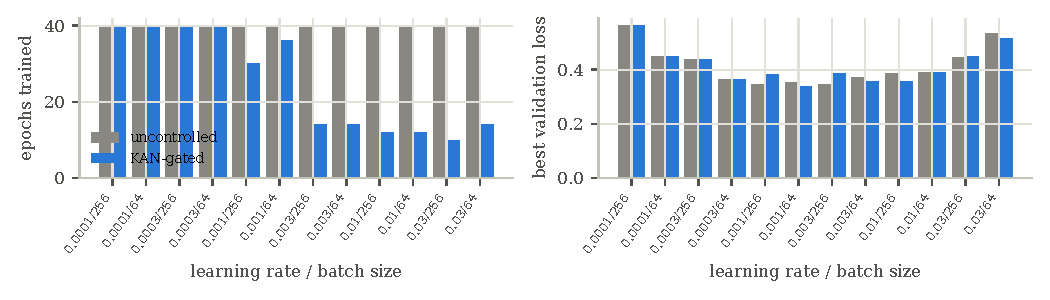
\includegraphics[width=0.85\textwidth]{figures/closed_loop.pdf}
\caption{Closed-loop control on 12 held-out configurations: epochs trained (left) and best validation loss (right), uncontrolled versus KAN-gated.}
\label{fig:closed}
\end{figure*}

The controlled runs used 302 of 480 epochs (37.1\% saved). Best validation loss was unchanged in aggregate: the median relative change was 0.0\% and the mean $+0.30\%$ (Wilcoxon $p=0.95$), with mean validation accuracy $+0.10$ points. Four runs improved by more than 0.5\%, all of them runs whose learning rate the gate had reduced (up to $-7.2\%$ at learning rate $10^{-2}$, batch 256); three got worse, two by $+10.6\%$ and $+11.1\%$ when a run that would still have improved was stopped after repeated reductions; five changed by less than 0.5\%. Low-learning-rate runs were left to finish.

Two behaviours are worth reporting. First, actuation latency: each controlled trajectory matched its uncontrolled twin exactly until one epoch after the first intervention, confirming that asynchronous control acts at the next epoch boundary. Second, the gate re-issues \emph{adjust LR} at consecutive checks while its score stays in the middle band, so the executor halved the learning rate up to ten times in one run. A cooldown between adjustments, or a gate input for recent interventions, is a straightforward fix that we leave to future work.


\subsection{Sensitivity to the tolerance}
The tolerance $\tau$ sets the trade-off. For gate seed 0, $\tau=2\%$, $5\%$ and $10\%$ give 27.8\%, 30.6\% and 38.1\% compute saved at 0.06\%, 0.15\% and 0.56\% mean regret, with premature-stop rates of 2.8\%, 5.6\% and 11.1\%. The linear gate follows the same trend (33.3\%, 35.8\%, 38.5\% saved at 0.28\%, 0.30\%, 0.64\% regret). $\tau$ is a single, interpretable knob: the relative improvement an operator is willing to forgo.

\section{Discussion and Limitations}
\textbf{What the KAN adds.} In this setting the KAN gate does not beat a linear gate or a well-chosen patience rule on efficiency. Its advantage is that its decision function is non-linear yet exact and readable, which allows an auditor to check what drives each decision and whether that structure is stable across retraining. Where a linear rule suffices, it should be preferred; the gate framework accepts either.

\textbf{Scale.} All results come from one small model, one dataset, a 40-epoch budget and CPU training; 36 runs bound the statistical power, and several differences that look sizeable are not significant. Generalisation to large models, long fine-tuning runs and other monitored metrics is untested.

\textbf{Repeated interventions.} The gate has no memory of its own past actions, so it can halve the learning rate at every check; Section~\ref{sec:closed} shows this both helping and hurting.

\textbf{Replay and labels.} Offline replay assumes the best checkpoint is retained and cannot evaluate learning-rate changes; hindsight labels for harvested runs are censored when the gate stops a run.

\textbf{System.} The LLM Supervisor ran in its deterministic fallback mode in our experiments (no API key), proposing the reference rule's action; because the gate is binding, this affects only logged agreement and the suggested learning rate. The budget feature is epoch-proportional rather than measured GPU time. The Kubeflow TrainJob client shares the tested interface but was not validated on a live cluster.

\section{Conclusion}
A symbolic KAN can serve as the binding decision layer of an agentic training controller, with decisions reproducible exactly from the displayed formula. The essential ingredient is the training signal: hindsight labels from completed real runs turn the gate from ineffective (4.4\% savings) into competitive (31.0\% savings at 0.20\% regret, near the oracle's regret). In closed loop it saves 37.1\% of epochs on held-out live runs without a significant change in best validation loss. Future work includes an intervention cooldown, larger models and fine-tuning workloads, measured GPU cost, cluster deployment on Kubeflow, uncertainty-aware stopping, and evaluating learning-rate interventions at scale.

\section*{Reproducibility}
Code, the 36 learning curves, benchmark outputs and this paper's figures are in the project repository (\texttt{experiments/}, \texttt{paper/}). Every number in Sections~V--VI is produced by \texttt{experiments/benchmark.py} and \texttt{experiments/closed\_loop.py}.

\bibliographystyle{IEEEtran}
\bibliography{refs}

\end{document}
